\documentclass[12pt,a4paper]{article}

\usepackage[english]{babel}
\usepackage{amsmath}
\usepackage{upgreek}
\usepackage{paralist}
\usepackage{verbatim}

\newcommand{\V}{\mathcal{V}}
\newcommand{\G}{\mathcal{G}}
% OSTblock
\newcommand{\B}{\mathcal{B}}
\newcommand{\BS}{\operatorname{BS}}
\newcommand{\BE}{\operatorname{BE}}
% State root
\newcommand{\SR}{\operatorname{SR}}
% Storage root
\newcommand{\SO}{\operatorname{SO}}
% OSTblock gas limit
\newcommand{\OL}{\operatorname{OL}}


% make in the latest NIPS format (as of this writing, 2017)

\usepackage[nonatbib,final]{nips_2017}
%\usepackage[nonatbib,final]{nips_2017}

\usepackage{color}
\usepackage{graphicx}
\DeclareGraphicsExtensions{.pdf,.eps,.png,.jpg}		% search for .pdf, then .eps, then .pngs, then .jpg

% look in these subdirectories for graphics referenced by \includegraphics
% each entry must end with a /
\graphicspath{{figs/}{figures/}{images/}{./}}

\newcommand*{\red}[1]{ \color{red} #1}

%\usepackage{tabularx}
\usepackage{url}
\usepackage{amsmath}

% this is for environments \subfigure and \subtable
\usepackage{subcaption}

% These packages are FORBIDDEN
%%%%%%%%%%%%%%%%%%%%%%%%%%%%%%%%%%%%%%%%%%%%%%%%%%%%%%%%
%\usepackage{lmodern} % messes up \textsc
%\usepackage{cite} % messes up NIPS
%\usepackage{fullpage} % messes up NIPS
%\usepackage{natbib} % messes up NIPS
%%%%%%%%%%%%%%%%%%%%%%%%%%%%%%%%%%%%%%%%%%%%%%%%%%%%%%%%

\usepackage{array}			% replacement for eqnarray.  Must be BEFORE \usepackage{arydshln}
\usepackage{units}			% for \nicefrac{\alpha}{\beta}


\usepackage{amsthm}		% for theorems
\newtheorem{definition}{Definition}

% text looks a little better
\usepackage{microtype}

\usepackage{wasysym}

\usepackage{textcomp, marvosym} % pretty symbols
\usepackage{booktabs} 	% for much better looking tables

% for indicator functions
\usepackage{dsfont}

% For automatic capitalizaton of section names, etc.
\usepackage{titlesec,titlecaps}


\Addlcwords{is with of the and in}
\Addlcwords{of the}
\Addlcwords{and}
\titleformat{\section}[block]{}{\normalfont\Large\bfseries\thesection.\;}{0pt}{\formatsectiontitle}
\newcommand{\formatsectiontitle}[1]{\normalfont\Large\bfseries\titlecap{#1}}

\titleformat{\subsection}[block]{}{\normalfont\large\bfseries\thesubsection.\;}{0pt}{\formatsubsectiontitle}
\newcommand{\formatsubsectiontitle}[1]{\normalfont\large\bfseries\titlecap{#1}}





% for pretty Euler script
% \usepackage[mathscr]{euscript}
% \usepackage{bold-extra}





%\usepackage{subfig}
\usepackage{float} % for \subfloat

%%%%%%%%%%%%%%%%%%%%%%%%%%%%%%%%%%%%%%%%%%
%% More customizable Lists
%%%%%%%%%%%%%%%%%%%%%%%%%%%%%%%%%%%%%%%%%%
% Better symbols custom enumerative lists, define any symbol you'd like
% \usepackage{enumitem}


%%%%%%%%%%%%%%%%%%%%%%%%%%%%%%%%%%%%%%%%%%
%% Custom Symbols 
%%%%%%%%%%%%%%%%%%%%%%%%%%%%%%%%%%%%%%%%%%
% \xspace at the end of custom macros never screws up spacing.
\usepackage{xspace}



%%%%%%%%%%%%%%%%%%%%%%%%%%%%%%%%%%%%%%%%
%% Abbreviations you'll always want
%%%%%%%%%%%%%%%%%%%%%%%%%%%%%%%%%%%%%%%%
\newcommand*{\TODO}[1]{{\centering {\small \sffamily \color{red} #1} \vskip10pt }}
\newcommand*{\todo}[1]{{\small \sffamily [{\color{red} #1}]}}
\newcommand*{\q}[1]{{\small \sffamily [{\color{blue} #1}]}}
\newcommand*{\fix}[1]{{\sffamily [{\textnormal{\color{red} #1}}]}}



%-----------------------------------------------------------------------------
%  Cross references
%-----------------------------------------------------------------------------
% The following code defines how you make references to figures, tables, etc...
% It is defined in one place only, and can be modified for all references
% in the document at the same time.
% Instead of typing each time: "see Fig. \ref{myfig}" you can create a command
% \figref which will do the job. Then in text you only type \figref{myfig} and LaTeX
% will do the rest.
\newcommand{\tblref}[1]{Table~\ref{#1}}
%\renewcommand*{\figref}[1]{Fig.~\ref{#1}}
\renewcommand{\eqref}[1]{eq.~(\ref{#1})}
\newcommand{\Subref}[1]{(\subref{#1})}


\newcommand{\figref}[1]{Figure~\ref{#1}}
\newcommand{\Figref}[1]{Figure~\ref{#1}}
\newtheorem{theorem}{Theorem}
\newtheorem{lemma}[theorem]{Lemma}

%%%%%%%%%%%%%%%%%%%%%%%%%%%%%%%%%%%%%%%%

% for \sout{} for strikeout
% \usepackage[normalem]{ulem}


% for better manipulation of tables
\usepackage{makecell}
\renewcommand\theadfont{\bfseries}


%-----------------------------------------------------------------------------
%  Misc symbols that I like
%-----------------------------------------------------------------------------
\newcommand*{\opname}[1]{\operatorname{#1}}


\renewcommand*{\to}{\rightarrow}


%%%%
\graphicspath{{images/}}

\title{Mosaic\\\sc\Large{Running Meta-Blockchains to Scale DApps}}
% TODO add all authors
\author{\textbf{Benjamin Bollen, Martin Schenck}\\ for OpenST Foundation \\ working draft}
\date{OpenST v0.10 - May 2018}

\begin{document}

\maketitle

% TODO check bibliography
\begin{abstract}
Mosaic is a set of Byzantine fault tolerant (BFT) meta-blockchains defined in smart contracts on Ethereum. A meta-blockchain has an open set of validators staked on Ethereum, and has a smart-contract based consensus engine.  Each block is committed by a super-majority vote. Mosaic introduces BFT consensus rules that allow validators to leverage more efficient auxiliary systems running in parallel for block production, while millions of transactions can be finalised before the header is asynchronously committed to Ethereum. Ethereum remains the sole source of truth by locking value tokens on Ethereum while minting a utility token representation on the auxiliary systems. Validators get rewarded collaboratively based on gas consumed thereby solving for the verifier’s dilemma. As a result Mosaic can finalise thousands of transactions per second on Ethereum at a lower gas price. We have built an atomic gateway protocol that Ethereum DApps can deploy to leverage Mosaic to scale.
\end{abstract}

%
% Section
%
\section{Introduction}
%Ethereum~\cite{ethereum} with its current proof of work Nakamoto consensus protocol is inherently limited in the number of transactions it can perform per second~\cite{verifiersdilemma}.
%In order for Ethereum to gain mass adoption, an increase in throughput is required.
%Current efforts include state channels~\cite{lightning} like the Raiden Network~\cite{raiden} and side chains~\cite{sidechains} like Plasma~\cite{plasma}.
%A drawback of the proposed solutions is the fact that the user has to be always online in order to ensure integrity of her transactions.
%Furthermore, in case of a mass exit, a congested Ethereum network could lead to lost funds.
%



%
% Section
%
%\section{Related Work}
%
%\paragraph{Verifiers' Dilemma}
%\cite{verifiersdilemma}
%
%\paragraph{Interblockchain Communication}
%\cite{cosmos}
%
%\paragraph{Casper FFG}
%\cite{casperffg}

%
% Section
%
%\section{Our Contribution}

%
% Section
%
\section{A mosaic of cores}

A meta-blockchain is defined in a smart contract by a genesis state, a staked validator set and consensus rules to progress the state.
%As layer one we assume a blockchain that has byzantine fault tolerance~\cite{pbft} and plausible liveliness~\cite{casperffg}.
%We call that blockchain \emph{Origin} $O$.
%We chose Ethereum as Origin for our first implementation.
%Transactions will take place on a sidechain that we call \emph{Auxiliary} $A$.
%Origin and Auxiliary must both % TODO what is it called that state is tracked and a state root exists?
%
%We assume Origin to track all ownership.
%Origin only lends ownership to Auxiliary.
%Thus, finality on Origin is always authoritative.
%If Auxiliary halts, users can recover the assets they own and there is no restriction in time for them to do so,
%enabling a coordinated mass exit over time.

%
% %% Objective
% Scale Etherum to thousands of transactions per second
% => Finalise thousands of transactions per second on Ethereum
%
% %% Origin
% Assume origin BFT and lively
%
% %% Method
% 1. Ownership model: Tokens and NFT
% 2. Borrow ownership onto auxiliary
%    Aux halts => non time-limited recovery
% 3. Origin finality is authoritative because ownership only borrowed 
%

% Somewhere say that we transfer state roots back and forth

\subsection{OpenST-Mosaic}
\label{subsec:mosaic}

% @benjaminbollen add intro

%Quote FFG slashing conditions and voting rules.

% General assumption
%Each validator can verify the blocks $a_i$ it has received (incomplete view).
%Origin is byzantine fault tolerant -> each validator can assert (prob) finality of the state of origin.

% See lemma plus accountability must be done twice in two directions

% TH 1 and 2 Vo can be slashed for the actions of Va

% All theorems and lemmas assume liveliness of Origin!!

%Theorem 1 and 2 assume known sets of validators
%Maybe theorem 1 is 1a and 1b
%1a simulated accountable safety
%1b simulated plausible liveliness


We assume without loss of generality that for every validator-address $v^O$ in the validator set $\V^O$ on origin a corresponding,
unique validator-address $v^A$ on auxiliary $A$ can be associated and we call the resulting validator set $\V^A$,
the validator set on $A$. A single actor is assumed to control and be responsible for both $v^O$ and the associated $v^A$.
On origin $v^O$ will always be held accountable for any signed message by $v^A$ on $A$, because and only $v^O$ has stake on origin.


\begin{lemma}[Remote Accountability]
	\label{lemma:remoteaccountability}
	A vote on $A$ that violates a Casper Commandment can be punished on $O$.
	\begin{proof}
		% TODO @benjaminbollen removed the lemma so we can not reference it anymore
		Given lemma~\ref{lemma:mapping}, a violation of either Casper Commandment can be proven on $O$ without the respective transaction residing on $O$.
		If a validator $\upnu^A$ published two distinct votes for the same target height, the relevant votes can be presented on $O$ and the signature can be validated.
		An offending validator $\upnu^O$ can be identified according to lemma~\ref{lemma:mapping} and its deposit slashed.
		The same is true if a validator $\upnu^A$ votes within the span of its other votes.
		All relevant votes including their signatures can be presented on $O$.
	\end{proof}
\end{lemma}

\begin{theorem}[Partial View]
	\label{theorem:partialview}
	Given Origin $O$ with blocks $b^{O}_i$, checkpoints $c^{O}_i$ can be reported on Auxiliary $A$, such that a set of validators $\V^O$ with stake on $O$ can reach finality about the reported checkpoints $c^{O}_i$ on $A$ as $\V^A$ with accountable safety enforced on $O$.
	\begin{proof}
		% TODO we need the block header from O
		% TODO we need to assume that validators can observe both chains
		% TODO mention that we need to trail O's head
		If you report checkpoints from Origin as $\left\langle h_c, h(c) \right\rangle$ where $h_c$ is the hash of any checkpoint c on Origin and $h(c)$ is the height of checkpoint c in Origin's checkpoint tree, then you can vote on Origin's checkpoints on Auxiliary according to the Casper FFG voting rules.
		A Casper FFG vote consists of two checkpoint hashes, two checkpoint heights, and the validator signature, all of which is now available on Auxiliary.
		
		Accountable safety is enforced according to lemma~\ref{lemma:remoteaccountability}.
		%(register checkpoints on Origin in order to prove Aux votes later?)
	\end{proof}
\end{theorem}

\begin{theorem}[Leveraged Security]
	\label{theorem:leveragedsecurity}
	Given that the auxiliary chain $A$ follows the Casper fork choice rule and
	given that the validators staked on Origin $O$,
	Casper can be applied to $A$ as a whole; without validators staking on $A$.
	It is not necessary to report blocks or block headers from $A$ to $O$.
	\begin{proof}
		% TODO
		Validators staked on Origin
		
		% TODO more precision
		Lemma~\ref{lemma:remoteaccountability} proves that the validators can be slashed on Origin for their actions on Auxiliary.
		Even though Auxiliary is not necessarily lively, Casper still has plausible liveliness,
		as Casper assumes that the underlying chain keeps producing blocks.
	\end{proof}
\end{theorem}

Reporting a finalised auxiliary checkpoint to Origin costs gas on Origin.
Therefore, validators do not have an incentive to copy the state root from Auxiliary to Origin.
We present an asynchronous mechanism that forces validators to copy the state root.
We define the amount of consumed gas since the last copied checkpoint $g$.
We define a limit of consumed gas $l$.
The finalised auxiliary checkpoint with the smallest dynasty where $g \geq l$ must be copied to Origin.
\begin{equation}
	\neg\exists f : h(f') < h(f) \land g(f') \geq l
\end{equation}

If the validators fail to copy that finalised checkpoint,
they are still incentivised to copy a later checkpoint to get rewarded (see below).
When a validator copies a state root of a later finalised checkpoint from Auxiliary to Origin,
then it can be proven that there exists a finalised checkpoint with a lesser height that is also above the gas limit.
To do that, a fisherman could present the earlier finalised checkpoint to Origin after the later one was committed.
The height, consumed gas, and validator signatures can be proven.
% TODO proof that they can be proven?
When that happens, all validators in the validator set are punished and the fisherman is rewarded.

We must track the consumed gas on Auxiliary in order to for this proof to work.

% TODO signatures can be combined into a tree and then each vO can verify it. Otherwise it can get too costly for a single party to report a block and get all signatures verified within one transaction

% What if Auxiliary does not have gas? We need gas in addition to a state root to be able to use Auxiliary.

% At this point we don't actually need the OSTblock concept. Only variable set of validators

% Should be in the "Rewards" section:
% we need to track all gas consumption
% validators get paid per gas

\begin{theorem}[Honesty Guard]
	\label{theorem:honestyguard}
	An honest validator will not be punished by the gas limit rules.
	\begin{proof}
		All validators, including the honest ones,
		would be punished if the lowest finalised auxiliary checkpoint above the gas limit were not reported to Origin.
		If there is at least one honest validator, however, that validator would report the auxiliary checkpoint to Origin.
		Thus, all validators get only punished if none of them is honest.
	\end{proof}
\end{theorem}

% TODO small reward for the reporter in order to mitigate parasitic behaviour

\begin{comment}
%
% %%
% %% Original Mosaic text below
% %%
%

\begin{theorem}[Accountable Safety]
\label{theorem:safety}
Two conflicting checkpoints $a_m$ and $b_n$ cannot both be finalized.
\begin{proof}
Let $a_m$ (with justified direct child $a_{m+1}$) and $b_n$ (with justified direct child $b_{n+1}$) be distinct finalized checkpoints as in.
\end{proof}
\end{theorem}
OpenST Mosaic enables chain-to-chain state transfer.
That allows us to secure an insecure chain's state on a secure chain.
We call the secure chain \emph{origin} $O$ and the insecure one \emph{auxiliary} $A$.
In order to be blockchain proposal mechanism agnostic,
we layer Casper~\cite{casperffg} on top of any auxiliary chain.
We apply Casper to auxiliary the same way its application to Ethereum is described in the paper.
We assume origin to have at least two properties:
practical byzantine fault tolerance (PBFT)~\cite{pbft} and plausible liveness~\cite{casperffg}.
Furthermore, we assume origin to have a concept of finality or at least economic finality.

Mosaic consists of Mosaic nodes that observe both $O$ and $A$
as well as a specific Gateway like the ones described in section~\ref{subsec:gateway}.
That means every Mosaic node runs a full node per chain,
an independent client software that observes both full nodes,
and there is one smart contract per chain that makes up the Gateway.

% TODO the following paragraph is misplaced, not all concepts are known
It is required to move state from auxiliary to origin in order for the state to be finalised.
State is only assumed to be final on origin,
as we do not assume any security properties of auxiliary.
On the other hand it is required to move state from origin to auxiliary,
because auxiliary must be made aware of the fact that its state has become final.
When we say that we transfer state,
we actually refer to the transfer of the root of the state tree.
Any state can be proven against a known root.
When we say that we transfer state between chains,
then we always assume an existing Gateway as described in section~\ref{subsec:gateway}.
That Gateway is used to transfer the root of state tree from one chain to another.

Mosaic \emph{Validators} are actors that vote on state that is transferred between the two chains.
In addition, on auxiliary, the Mosaic validators also take the role of the Casper~\cite{casperffg} validators.
Their deposit, however, is only a single deposit for all actions and it is stored solely on origin.
Similarly to Casper, any Mosaic validator's deposit rises and falls with rewards and penalties, respectively.
When we say "$\frac{2}{3}$ of validators", we equally refer to the deposit-weighted fraction.

The set of Mosaic validators needs to be able to change.
The logic is similar to that of Casper with the notable difference that, instead of dynasties, we use OSTblocks (described below).
When a potential validator sends a \emph{deposit message} on origin at OSTblock height $\alpha$,
then the validator will be announced as part of the next set of validators in the header of OSTblock $\alpha+1$ and 
the validator $\upnu$ will join the validator set at OSTblock height $\alpha+2$.
% TODO a lot copied from Casper. OK? Required?
Analogous to Casper, we call $\alpha+2$ the validator's \emph{start OSTblock}, $\BS(\upnu)$.
If a validator $\upnu$'s withdraw message is included on origin's blockchain during an open OSTblock $\B_\alpha$,
it similarly leaves the set of validators at OSTblock height $\alpha+2$.
We call $\alpha+2$ the validator $\upnu$'s \emph{end OSTblock} $\BE(\upnu)$.

% TODO inparaenum not clear enough; maybe split it into paragraphs
Mosaic validators can vote on a number of events:
\begin{inparaenum}[(a)]
	\item origin state transfers to auxiliary,
  	\item auxiliary state transfers to origin and
	\item checkpoint justifications on auxiliary in the role of a Casper validator.
\end{inparaenum}
On auxiliary, checkpoints are justified and finalised by supermajority links as described in Casper.
Origin's (economical) finality is assumed as a given.
Thus, state is final on its respective chain and only the transfer must be must be approved on the other chain.
When state is transferred between the two chains, in any direction,
a simple $\frac{2}{3}$ majority vote on that state successfully commits it to the receiving chain.
A committed state that is (economically) finalised is regarded as finalised on the receiving chain.

\emph{OSTblocks} are a compressed representation of auxiliary's transactions.
% TODO are OSTblocks' transactions blocks or dynasties from auxiliary?
% TODO do OSTblocks include forks or only the canonical chain of auxiliary (redundant if we only store latest state)
Transactions in an OSTblock each represent one block of the auxiliary chain.
An OSTblock transaction represents the state change from the beginning of its associated block to the end of that block.
Therefore, OSTblocks are generated at a slower pace.
We call $\alpha$ the height of OSTblock $\B_\alpha$.
The next OSTblock, that points to $\B_\alpha$ in its header,
is OSTblock $\B_{\alpha+1}$ at height $\alpha+1$.
Due to the aforementioned compression of blocks on auxiliary,
$\B_\alpha$ may contain auxiliary blocks $b_{A{}i}$ to $b_{A{}i+m}$,
which means any number $m$ of blocks,
where $b_{A{}i+m}$ must be a Casper checkpoint that has been finalised on auxiliary.

The OSTblock header of block $\B_alpha$ at height $\alpha$ contains:
\begin{enumerate}
	\item A link to the previous OSTblock
	\item The signatures of the Mosaic validators in $\V_\alpha$
	\item The state root of the last block of auxiliary that is contained within the OSTblock
	\item The set of Mosaic validators for the next OSTblock, $\V_{\alpha+1}$
\end{enumerate}
The body of an OSTblock consists of all the transactions that make up the blocks on auxiliary that are contained within this OSTblock.
We do not store the body of an OSTblock on origin, only the header.
The body can be re-created at any time from the auxiliary chain and proven against auxiliary's state root that is securely stored on origin.

We consider an OSTblock \emph{closed,} when the full header with the state root from auxiliary is committed to origin.
We consider an OSTblock \emph{opened,} when the new OSTblock header has been transferred to auxiliary.

% TODO language whole paragraph; also duplicate
In order to be block proposal mechanism agnostic, we layer Casper~\cite{casperffg} on top of auxiliary.
% TODO missing context. Extend or move to validators paragraph above
Validators vote on supermajority links.
Auxiliary must follow Casper's fork choice rule.
% TODO missing context
Checkpoints get finalised.
The Mosaic validators can transfer the state of a finalised auxiliary checkpoint to origin.
% TODO language
A validator uses the Mosaic Gateway to transfer the state to origin.
On origin, a $\frac{2}{3	}$ majority vote is required by the validators in order to commit the state to origin.
% TODO how do we trigger this info back to aux?
The state is regarded economically finalised when the block that contains the commit is considered economically final on origin.

\begin{figure}[htb]
    \centering
	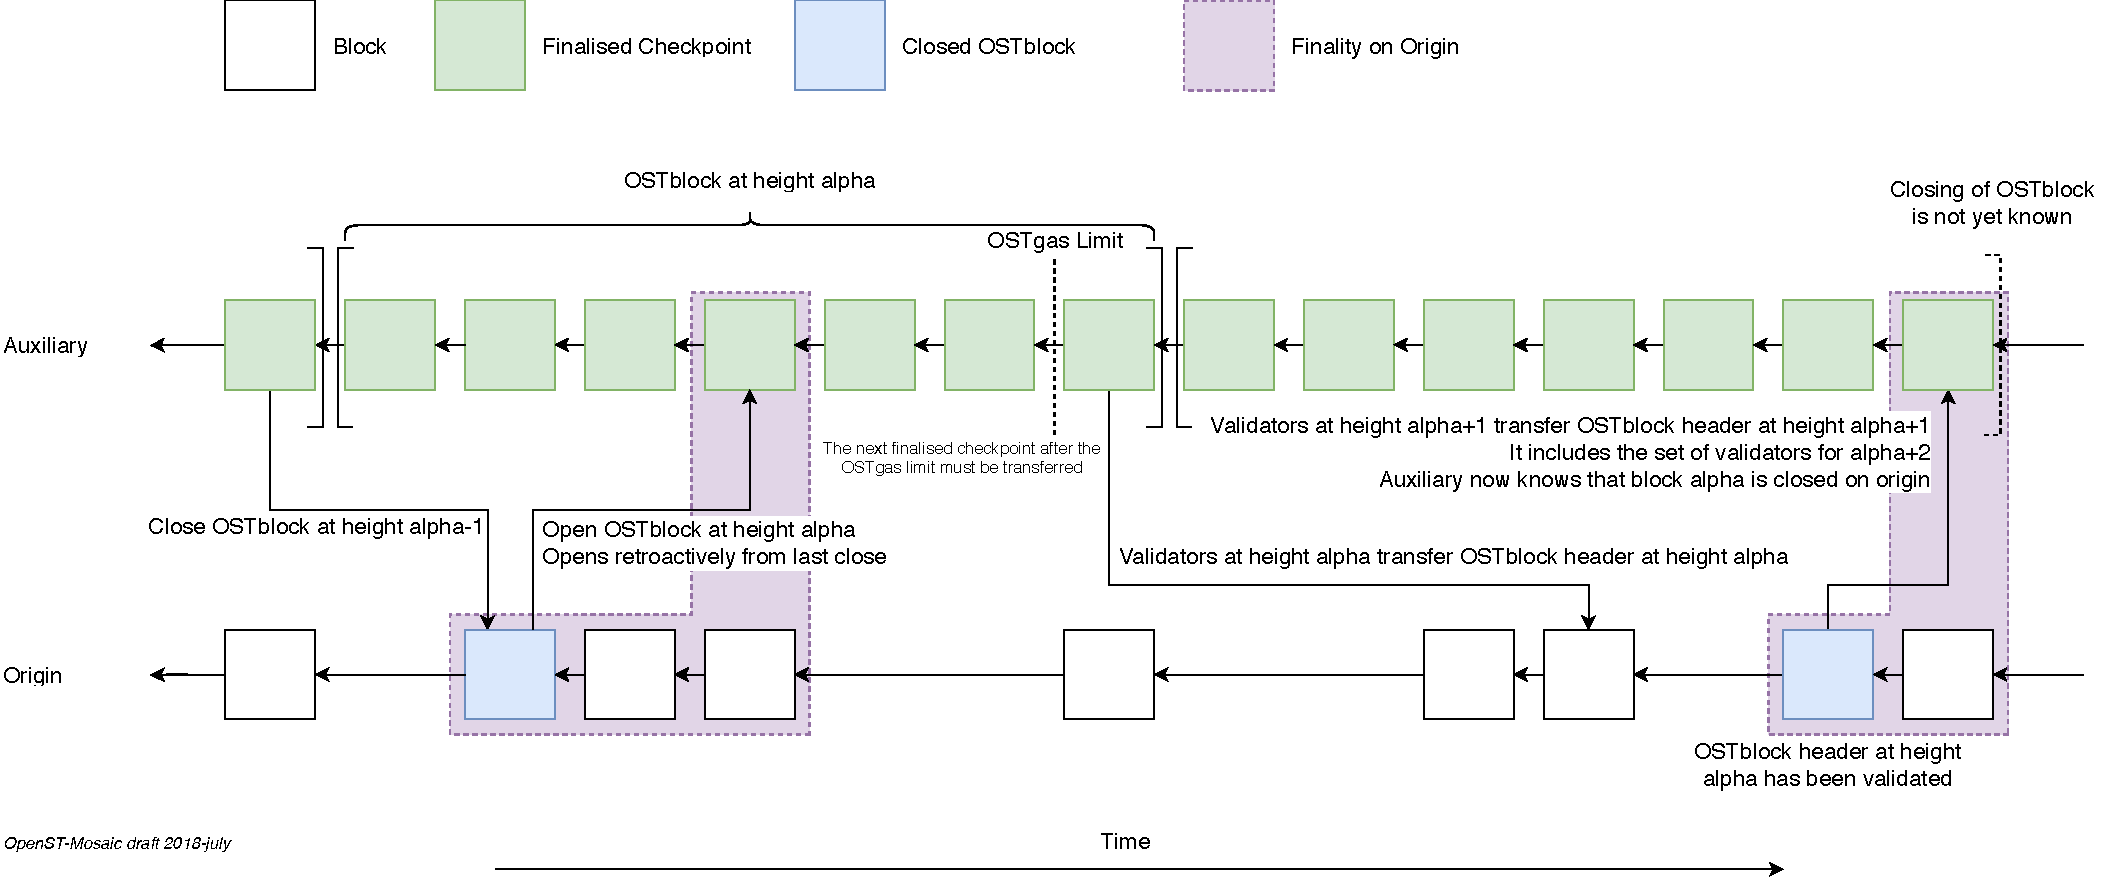
\includegraphics[width=\textwidth]{mosaic}
	\caption{\textbf{The Mosaic state transfer.}
		The closing of $\B_{\alpha-1}$ means that the finalised checkpoint $b_{A{}i}$ is the last block of $\B_{\alpha-1}$.
		Even though the details of $\B_\alpha$ will not be known until the opening is transferred to $A$,
		the first block in $\B_\alpha$ will be $b_{A{}i+1}$.
		Once a checkpoint is finalised after the OSTgas limit has been reached,
		% TODO V or a Mosaic node? where's the difference?
		$\V$ will signal the closing of $\B_\alpha$ to $O$.
	}
	\label{fig:mosaic}
\end{figure}

% TODO extend this paragraph
On the auxiliary chain, \emph{OSTgas} is the equivalent to gas on Ethereum.
For transactions to be included in blocks on auxiliary, a fee is paid for the consumed OSTgas.

% TODO possibly move this further up
Mosaic validators are allowed to commit every finalised state from auxiliary to origin.
However, that may be infeasible from an economic viewpoint of the validators.
Therefore, we propose points on the auxiliary chain where the validators must close the OSTblock.
Whenever a certain fixed limit of OSTgas has been spent on auxiliary since the opening of the OSTblock,
the validators \emph{must} close the OSTblock at the next finalised auxiliary checkpoint.
If a validator does not vote to commit that checkpoint,
its deposit can be slashed.
The OSTgas limit is marked in figure~\ref{fig:mosaic} by the dashed line.

Actors on the auxiliary chain have an economic incentive to finalise their state on origin.
The block creators of auxiliary will pay a fraction of their earned OSTgas to the Mosaic validators as a fee when the validators move the state to origin.
% TODO context and language
% TODO why?
Due to the OSTblocks, Mosaic validators can only copy the state from auxiliary to origin after the state of origin has been copied to auxiliary.
Thus, validators are incentivised to close an OSTblock and open a new one in order to earn the OSTgas fee for the transfer of auxiliary's state.

% TODO extend paragraph on punishment
It must be possible to hold Mosaic validators accountable if they misbehave.
In order to do so, anyone must be able to present proof of malicious actions on origin,
as the validators' deposits are stored there.
When a validator violates a slashing condition on auxiliary by making an illegal vote,
that fact is stored in the state of auxiliary.
Therefore, it can be proven against the state root of auxiliary.
Since the state root of auxiliary is available on origin,
the proof and the subsequent slashing can be carried out on origin as well.

% TODO extend paragraph on long range revisions
To prevent long range revisions, we apply the same rules that Casper applies:
after a Mosaic validator leaves the set of validators, its deposit is kept for another four months.
Casper votes on auxiliary can only be carried out up to three months into the past.
That leaves one month headroom to blame auxiliary's adversaries on origin and get its deposit slashed.
\end{comment}

\subsection{OpenST-Gateway}
\label{subsec:gateway}

OpenST Gateway enables chain-to-chain transfer of state objects.

\subsection{Reward Structure}
On Origin in OST.

rewarding for reported block headers that get finalised

\subsection{Dynamic Set of Validators}

\subsection{Set-Up of An Auxiliary Chain}
Start running with gas cost of 0.
Set up contract with base token.
Set up Gateways, but closed.
Give one week of blaming on Origin. How can there be proof on Origin without Aux's state root? Or is that also transferred in the set-up phase? If so: why is it trusted?
Open Gateways.

%
% Section
%
\section{Outlook}

\subsection{Token Economies}
\subsection{Neo and Cardano}

%
% Section
%
\section{Conclusion}

\bibliographystyle{naturemag}
\bibliography{openst}

\end{document}
